\documentclass[border=10pt]{standalone}
\usepackage{pgfplots}
\pgfplotsset{compat=1.18}
\begin{document}
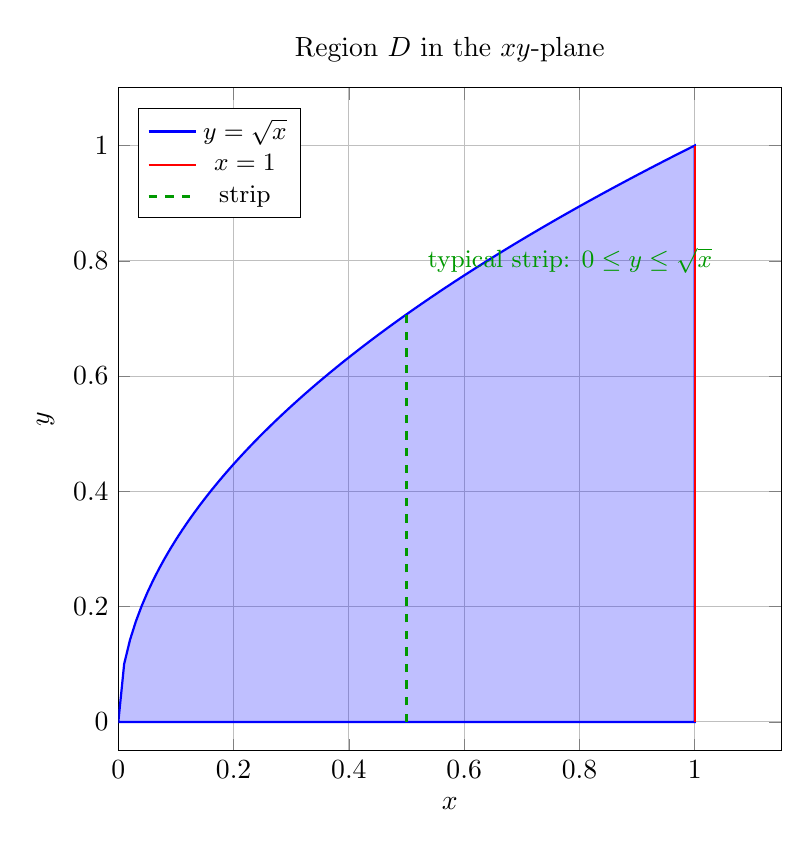
\begin{tikzpicture}
\begin{axis}[
    width=10cm, height=10cm,
    xlabel={$x$}, ylabel={$y$},
    xmin=0, xmax=1.15, ymin=-0.05, ymax=1.1,
    grid=both,
    axis equal image,
    title={Region $D$ in the $xy$-plane},
    legend style={at={(0.03,0.97)}, anchor=north west, font=\small},
]
% filled region D under y = sqrt(x)
\addplot+[domain=0:1, samples=100, draw=blue, fill=blue, fill opacity=0.25, draw opacity=1, thick, mark=none] {sqrt(x)} \closedcycle;
% x = 1 boundary
\addplot[red, thick, mark=none] coordinates {(1,0) (1,1)};
% typical strip
\addplot[green!60!black, dashed, very thick, mark=none] coordinates {(0.5,0) (0.5,0.7071)};
\node[green!60!black, anchor=west, font=\small] at (axis cs:0.52,0.8) {typical strip: $0\leq y\leq\sqrt{x}$};
\legend{$y=\sqrt{x}$, $x=1$, strip}
\end{axis}
\end{tikzpicture}
\end{document}